The data collected in the experiments requires further processing before feature extraction and classification are made. This section describes the process of data collection and data preprocessing in detail. Data preprocessing is needed in order to present the micro-Doppler signatures and attenuate the background noise.
\subsection{Data collection}
With the Doppler radar system described in Section II, radars signals were collected and stored in a database. As illustrated in Fig. \ref{fig_dfd}, signals collected by the BumbleeBee radars were transferred to the TelosB nodes and radio transferred to the TelosB base station. The TelsoB base station was connected to a computer which received the signals through a serial port. Finally, all data was stored into a MongoDB database system, which is an open source NoSQL database and it is usually utilized to store a large amount of time series data.
\begin{figure}[h]
\centering
%\captionsetup{justification=centering}
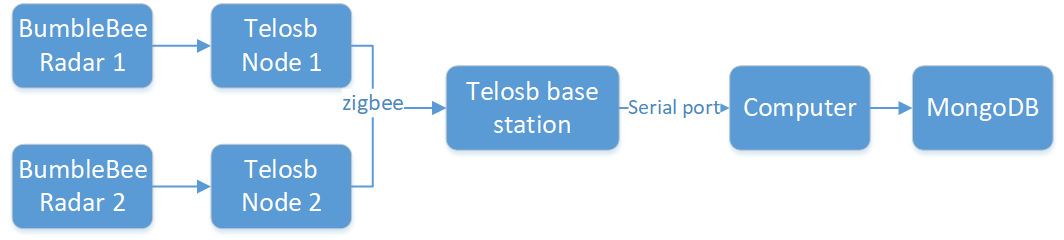
\includegraphics[width=3.4in]{dfd}
\caption{Data flow diagram of Doppler radar signals}
\label{fig_dfd}
\end{figure}

The final data stored into the database contains not only radar signals, but also labels that informed the time, the types of the target and the types of human activities (walking or running), etc. Table I shows the information of each field of a radar signal recorded in our MongoDB system. The sample frequency of the radars is 250 Hz. The data collected in the experiments were used to train the classifiers. In prediction, only the ID of the signals, I and Q values, and the time were used.
\begin{table}[]
\centering
\caption{Fields of the signal collection}
\label{tab_field}
\begin{tabular}{|l|l|}
\hline
\textbf{Field} & \textbf{Information}                                                                                                                           \\ \hline
ID             & The identity number of a Doppler radar signal                                                                                                  \\ \hline
Q              & The quadrature power value of a signal                                                                                                         \\ \hline
I              & The in-phase power value of a signal                                                                                                           \\ \hline
Time           & \begin{tabular}[c]{@{}l@{}}The time a signal was collected (accurate to a millisecond)\end{tabular}                                \\ \hline
SubjectType    & \begin{tabular}[c]{@{}l@{}}The type of a target or targets. `0` is human, `1` is dog, \\`2` is human and dog, `3` is no target.\end{tabular}  \\ \hline
SubjectID      & The ID of the targets.                                                                                                                         \\ \hline
SubjectNum     & The number of participants as a target.                                                                                                                     \\ \hline
Activity       & \begin{tabular}[c]{@{}l@{}}The type of human activity. `0` is walking,\\  `1` is running, `2` is no human activity\end{tabular}                \\ \hline
Angle          & \begin{tabular}[c]{@{}l@{}}The angle between the direction of human movement and\\ the radar beam.\end{tabular}                               \\ \hline
Range          & \begin{tabular}[c]{@{}l@{}}The range of the target located in. ‘0’ is 1-3m, \\ ‘1’ is 3-5m, ‘2’ is 5-8m, ‘3’ is not in any range.\end{tabular} \\ \hline
RadarNum       & \begin{tabular}[c]{@{}l@{}}The number of radars used in the system set up: 2.\end{tabular}               \\ \hline
NodeID         & \begin{tabular}[c]{@{}l@{}}The ID of primary node that consists of \\ BumbleBee 1 and Telsob 1 here.\end{tabular}                              \\ \hline
SecNodeID      & \begin{tabular}[c]{@{}l@{}}The ID of secondary node that consists of \\ BumbleBee 2 and Telsob 2 here.\end{tabular}                            \\ \hline
\end{tabular}
\end{table}

\subsection{Data preprocessing}
The original signal is a complex value ($I+jQ$). $I$ is the real part and $Q$ is the imaginary part. Micro-Doppler signatures are represented in a time-frequency domain. It is required to transform the original radar signals from the time-amplitude domain into the time-frequency domain using STFT. Fig. \ref{fig_dp}(b) shows a spectrogram generated by STFT. However, the spectrogram suffers from a band of heavy clutter between +/- 5 Hz. The clutter makes the fluctuations obtained from the human walking quite fade. In order to attenuate the clutter, a Butterworth high-pass filter is applied to the raw signals. The Butterworth high-pass filter can be represented by the following equation \cite{dogra2014image}:
\begin{equation}
\label{eq_butter}
\left | H(w) \right |^2=1/(1+(w/w_c )^{2n} )=1/(1+\varepsilon ^2 (w/w_s )^{2n} ),
\end{equation}
where $n$ is the order of filter, $w_c$ is the cutoff frequency (5 Hz here), $w_s$ is the stopband boundary frequency.

After filtering, a new spectrogram is generated as it can be seen in Fig. \ref{fig_dp}(c). The fluctuations obtained from human movements are now more distinctive. Note the spine of the plot corresponds to the motion from the torso, the smaller fluctuations around the spine corresponds to the motions from arms and legs. Positive and negative Doppler frequencies correspond to the subject moving toward or away from the radar, respectively. However, the high-pass filter is only used to attenuate parts of the clutter and noise that are below $w_c$. For improving the robustness of the classifiers, the samples are required to be collected from environments with high-levels of clutter. By training the classifiers with those samples, they can learn how to reduce the interference of the noise in the environment.
\begin{figure}[!t]
\centering
%\captionsetup{justification=centering}
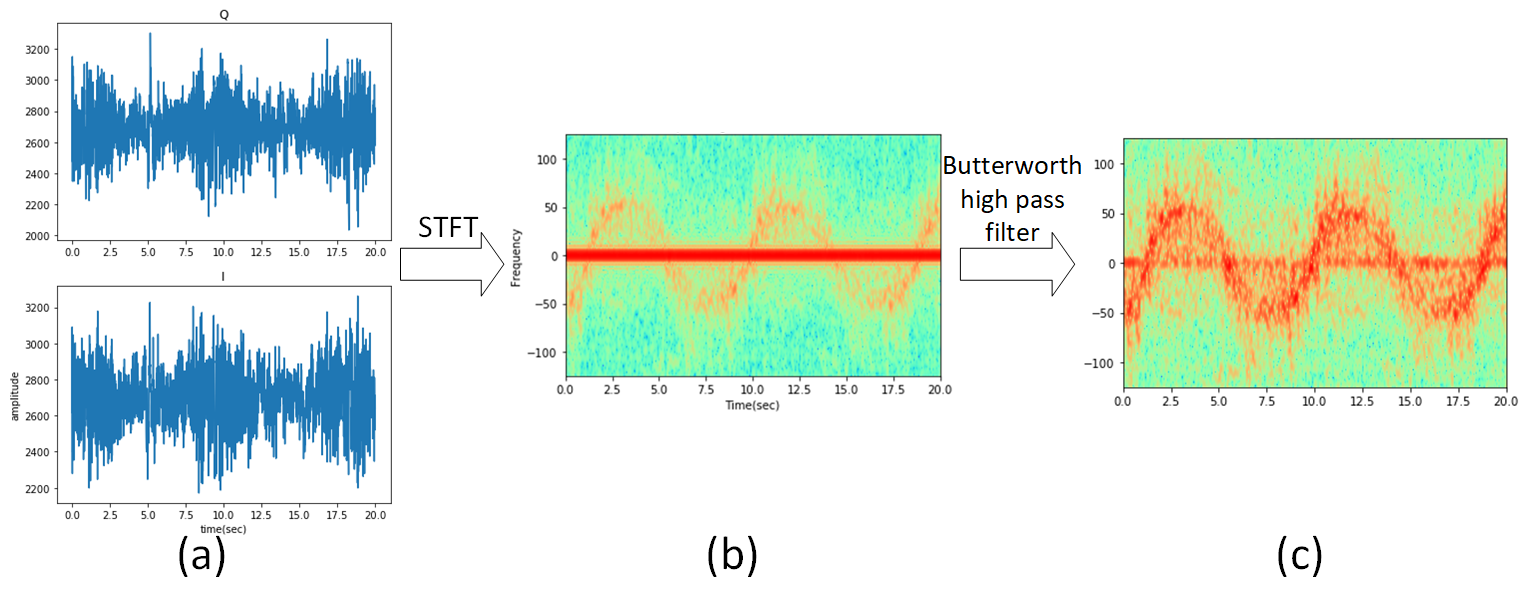
\includegraphics[width=3.4in]{data_processing}
\caption{Data preprocessing, (a) original signals, (b) spectrogram after STFT, (c) spectrogram after high-pass filter}
\label{fig_dp}
\end{figure}

With the STFT technique, a different length of a sequence will result in a different width of the frequency spectrogram. A windowed short time FFT processing technique with a window length of 64 samples and a Hanning weighting, transforms a sequence of 2500 signal samples into a frequency spectrogram with the size of $2048\times 304\times 1$ (2048 is the height, 304 is the width, 1 is the depth). The frequency spectrogram can be taken as an image with one channel. Fig. \ref{fig_sliding} presents a frequency spectrogram that was created from a sliding-window with the window size of 2500 frames (2500 samples within the sliding window) and the sliding step with the length of 100 frames. The sampling frequency of the micro-Doppler signals is 250Hz. So by moving the sliding-window with continuous sliding steps, a spectrogram can be extracted at every 0.4 seconds, which is calculated by $(Sliding\; step \;length)/(sample\; frequency)$, i.e. $100/250$. The effect of the window size is investigated in Section IX.
\begin{figure}[!t]
\centering
%\captionsetup{justification=centering}
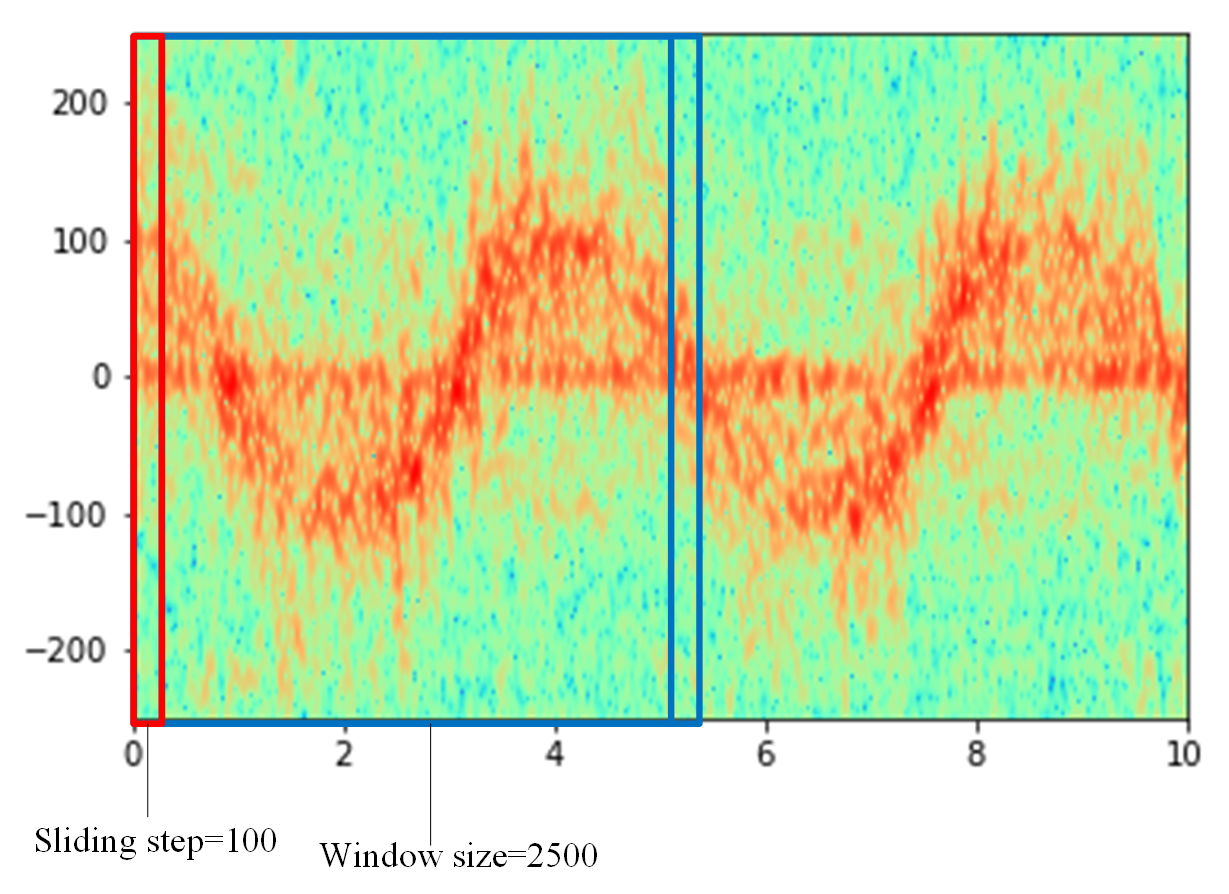
\includegraphics[width=3.4in]{sliding}
\caption{A sliding window of STFT}
\label{fig_sliding}
\end{figure}

Through the above processing methods and using an STFT sliding window of 1250 frames (time length of 5s), the described experiments generated 46900 spectrograms in total. The composition of the samples/spectrograms is shown in Table \ref{tb-sample}.
% Please add the following required packages to your document preamble:
% \usepackage{multirow}
\begin{table}[]
\centering
\caption{The composition of samples}
\label{tb-sample}
\begin{tabular}{|c|c|c|c|c|}
\hline
\textbf{Subject}               & \textbf{Angle} & \textbf{Walking} & \textbf{Running} & \textbf{Total}         \\ \hline
\multirow{3}{*}{Single person} & 0°             & 1150             & 1200             & \multirow{3}{*}{15400} \\ \cline{2-4}
                               & 45°            & 2700             & 3150             &                        \\ \cline{2-4}
                               & 90°            & 3500             & 3700             &                        \\ \hline
\multirow{3}{*}{Two people}    & 0°             & 550              & 550              & \multirow{3}{*}{7000}  \\ \cline{2-4}
                               & 45°            & 1600             & 1550             &                        \\ \cline{2-4}
                               & 90°            & 1150             & 1600             &                        \\ \hline
\multirow{3}{*}{Three people}  & 0°             & 600              & 550              & \multirow{3}{*}{7200}  \\ \cline{2-4}
                               & 45°            & 1250             & 1700             &                        \\ \cline{2-4}
                               & 90°            & 1300             & 1800             &                        \\ \hline
\multirow{3}{*}{Four people}   & 0°             & 500              & 550              & \multirow{3}{*}{6950}  \\ \cline{2-4}
                               & 45°            & 1200             & 1650             &                        \\ \cline{2-4}
                               & 90°            & 1150             & 1900             &                        \\ \hline
Dog                            & 90°            & \multicolumn{2}{c|}{1350}           & 1350                   \\ \hline
\multirow{2}{*}{Human and Dog} & 0°             & \multicolumn{2}{c|}{1200}           & \multirow{2}{*}{3150}  \\ \cline{2-4}
                               & 90°            & \multicolumn{2}{c|}{1950}           &                        \\ \hline
Background                     & \multicolumn{3}{c|}{}                                & 5850                   \\ \hline
\end{tabular}
\end{table}


For the classification, the samples were separated into two groups, 80\% of the samples were used for training and validation, and 20\% for testing. As it can be seen from Table \ref{tb-sample}, the sample size for the classes is not balanced. In order to overcome this problem, different weights were assigned to each class in the training process; and the weight ratio was inversely proportional to the proportion of spectrograms of the various classes. However, for human recognition, because the numbers of spectrograms of the experiments with humans and the background are far greater than the number of spectrograms of the experiments with a dog (including human and dog), we randomly selected 2000 spectrograms of human and 2000 spectrograms of the background for the training.

In the training process, a 10-fold cross-validation has been applied; the samples/spectrograms for training and validation are further split randomly into 10 subsets without replacement. In each training iteration, nine subsets are used for training and one subset is used for validation.